\documentclass[12pt]{article}
\usepackage{geometry}                % See geometry.pdf to learn the layout options. There are lots.
\geometry{letterpaper}                   % ... or a4paper or a5paper or ... 
%\geometry{landscape}                % Activate for for rotated page geometry
\usepackage[parfill]{parskip}    % Activate to begin paragraphs with an empty line rather than an indent
\usepackage{daves,fancyhdr,natbib,graphicx,dcolumn,amsmath,lastpage,url}
\usepackage{amsmath,amssymb,epstopdf,longtable}
\usepackage{paralist}  % need to properly formulate standard answer blocks
\usepackage[final]{pdfpages}
\DeclareGraphicsRule{.tif}{png}{.png}{`convert #1 `dirname #1`/`basename #1 .tif`.png}
\pagestyle{fancy}
\lhead{CE 3305 Fluid Mechanics; Exercise Set 5}
\rhead{Name:\_\_\_\_\_\_\_\_\_\_\_\_\_\_\_\_\_\_\_\_\_\_\_\_\_\_\_\_\_\_\_\_\_\_}
\lfoot{REVISION A}
\cfoot{}
\rfoot{Page \thepage\ of \pageref{LastPage}}
\renewcommand\headrulewidth{0pt}
%%%%%%%%%%%%%%%%%%%%%%%%%%%%%%%%%%%%
\begin{document}
%%%%%%%%%%%%%%%%%%%%%%%%%%%%%%%%%%%
\begingroup
\begin{center}
{\textbf{{ CE 3305 Engineering Fluid Mechanics} \\ Exercise Set 5 \\ Summer 2018 -- GERMANY} }
\end{center}
\endgroup
\begingroup
~\newline
\textbf{Purpose} : Pressure variation in layered fluids of different densities.  Manometry used to determine density of unknown fluid.\\
\textbf{Assessment Criteria} : Completion, plausible answers, use of \textbf{R} for calculations. \\~\\
\textbf{Exercises} :

\begin{enumerate}
\item (Problem 3.16 pg 96)
Figure \ref{fig:AirOilWaterTank} is a schematic of a closed tank with Bourdon-tube gages tapped into it.   
\begin{enumerate}[a)]
\item What is the specific gravity of the oil?
\item What is the pressure reading on gage C?
\end{enumerate}
\begin{figure}[htbp] %  figure placement: here, top, bottom, or page
   \centering
   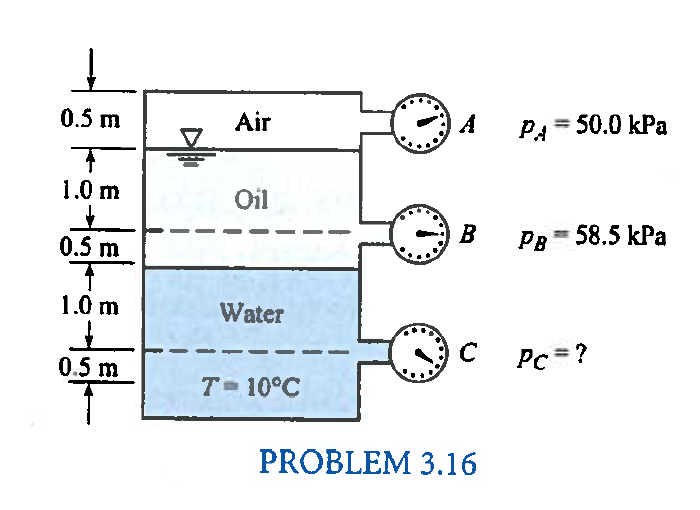
\includegraphics[width=3in]{AirOilWaterTank.jpg} 
   \caption{Closed tank with three phase system (Air, Oil, Water)}
   \label{fig:AirOilWaterTank}
\end{figure}
\clearpage

\item (Problem 3.54 pg 101)
A device for measuring the specific weight of a liquid consists of a YouTube manometer as depicted in Figure \ref{fig:YouTubeManometer}.
The manometer tube has an internal diameter of 0.5 cm and originally has water in it.
Exactly 2 cm$^3$ of unknown liquid is poured into one leg of the manometer, and a displacement of 5 cm is measured between the free surfaces as shown.  What is the specific weight of the unknown liquid?
\begin{figure}[htbp] %  figure placement: here, top, bottom, or page
   \centering
   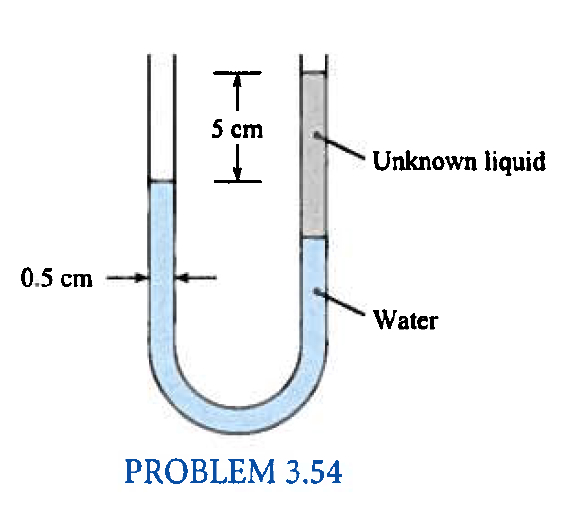
\includegraphics[width=2in]{YouTubeManometer.jpg} 
   \caption{U-Tube manometer for measuring specific weight}
   \label{fig:YouTubeManometer}
\end{figure}

~
\end{enumerate}


\end{document}  